\subsubsection{Stackgres mit Citus}
\begin{flushleft} 
    Stackgres ist eine PostgreSQL Implementation die dafür vorgesehenen ist, in einem Kubernetes Cluster betrieben zu werden.
\end{flushleft} 
\begin{flushleft}
    An sich wäre Stackgres nur eine Implementation von Patroni in Kubernetes inkl.
    Load Balancer.\\
    Nun kommt das Citus-Plugin ins spiel, welches aus einer jeden Monolithischen, klassischen PostgreSQL Installation eine Distributed SQL Umgebung macht.
\end{flushleft}
\begin{flushleft}
    Citus Data, der Entwickler von Citus, wiederum ist in den Microsoft Konzern eingebettet
\end{flushleft}
\begin{flushleft}
    \paragraph{Core-Features}
    Die wichtigsten Features von Stackgres sind\cite{G3XQA8PI}:
    \begin{itemize}
        \item k8s integration
        \item Deklaratives k8s CRD
        \item Autoamtische Backups
        \item Grafana und Prometheus integration
        \item Management Web Konsole
        \item Erweiterte Replikationsmöglichkeiten
        \item Integriertes Pooling
        \item Integrierter Proxy
    \end{itemize}
\end{flushleft}
\begin{flushleft}
    \paragraph{Replikation}
    Stackgres bietet Asynchrone und Synchrone Replikation, Gruppenreplikation sowie kaskadierende Replikation an.
\end{flushleft}
\begin{flushleft}
    Citus bietet sein eigenes Modell mit dem Sharding an.
\end{flushleft}
\begin{flushleft}
    \paragraph{Proxy}
    Stackgres hat den Proxy bereits mit envoy\cite{QAGSHVBL} implementiert.
\end{flushleft}
\begin{flushleft}
    \paragraph{Pooling}
    PgBounder\cite{ATBELZ2X} ist bereits integriert, es braucht also keinen weiteren Pooler.
\end{flushleft}
\begin{flushleft}
    \paragraph{API / Skripte}
    Stackgres wird Primär über YAML-Files und Kubernetes gesteuert, bietet aber eine eigene API an.
\end{flushleft}
\begin{flushleft}
    Citus bietet ebenfalls eine eigene API, mit der Citus vollständig verwaltet werden kann.
\end{flushleft}
\begin{flushleft}
    \paragraph{Architektur}
    \begin{flushleft}
        \subparagraph{StackGres}
        Stackgres packt PostgreSQL, Patroni, PgBouncer und envoy in einen Kubernetes Pod:
        \begin{figure}[H]
            \centering
            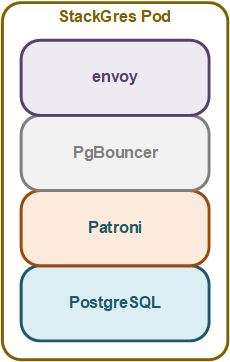
\includegraphics[width=0.75\linewidth]{source/implementation/evaluation/postgresql_ha_solutions/stackgres/stackgres_pod_architecture}
            \caption{Stackgres - Grundarchitektur}
            \label{fig:stackgres_pod_architecture}
        \end{figure}
    \end{flushleft}
    \begin{flushleft}
        \subparagraph{Citus Coordinator und Workers}
        Citus arbeitet mit einem Coordinator-Node, der jedes Query analysiert und an einen Worker-Node weitergibt.
        \begin{figure}[H]
            \centering
            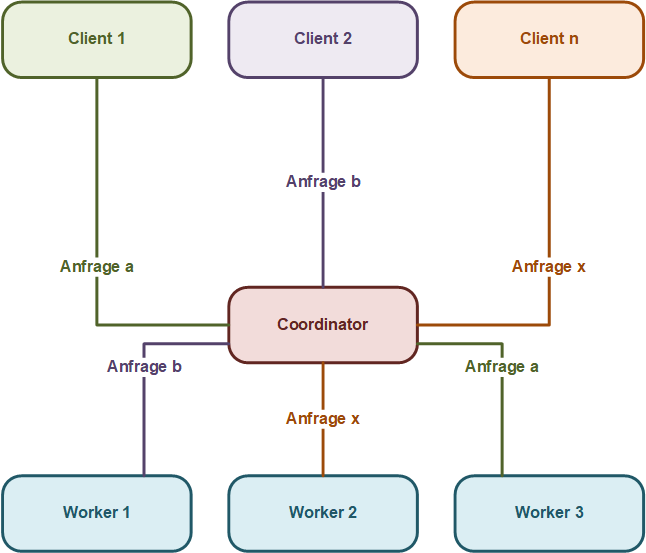
\includegraphics[width=0.75\linewidth]{source/implementation/evaluation/postgresql_ha_solutions/stackgres/citus_coordinator_worker}
            \caption{Citus - Coordinator und Workers}
            \label{fig:citus_coordinator_worker}
        \end{figure}
    \end{flushleft}
    \begin{flushleft}
        \subparagraph{Citus Sharding}
        Citus bietet zwei Sharding-Modelle an.
        \begin{flushleft}
            \textbf{Row-based sharding}
            Beim diesen sharding werden Tabellen anhand einer Distribution Column aufgeteilt. \cite{2Y5FA36C, FDUUL9IM}
            \begin{figure}[H]
                \centering
                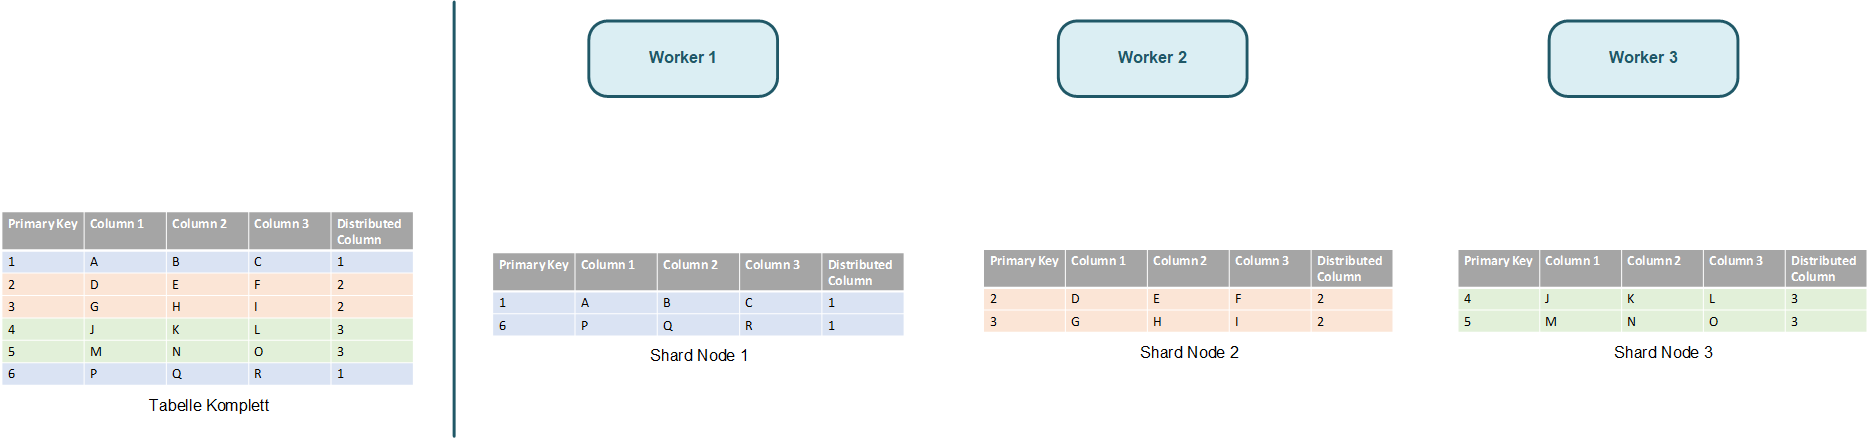
\includegraphics[width=0.8\linewidth]{source/implementation/evaluation/postgresql_ha_solutions/stackgres/citus_row-based-sharding}
                \caption{Citus - Row-Based-Sharding}
                \label{fig:citus_row-based-sharding}
            \end{figure}
        \end{flushleft}
        \begin{flushleft}
            \textbf{Schema-based sharding}
            \begin{figure}[H]
                \centering
                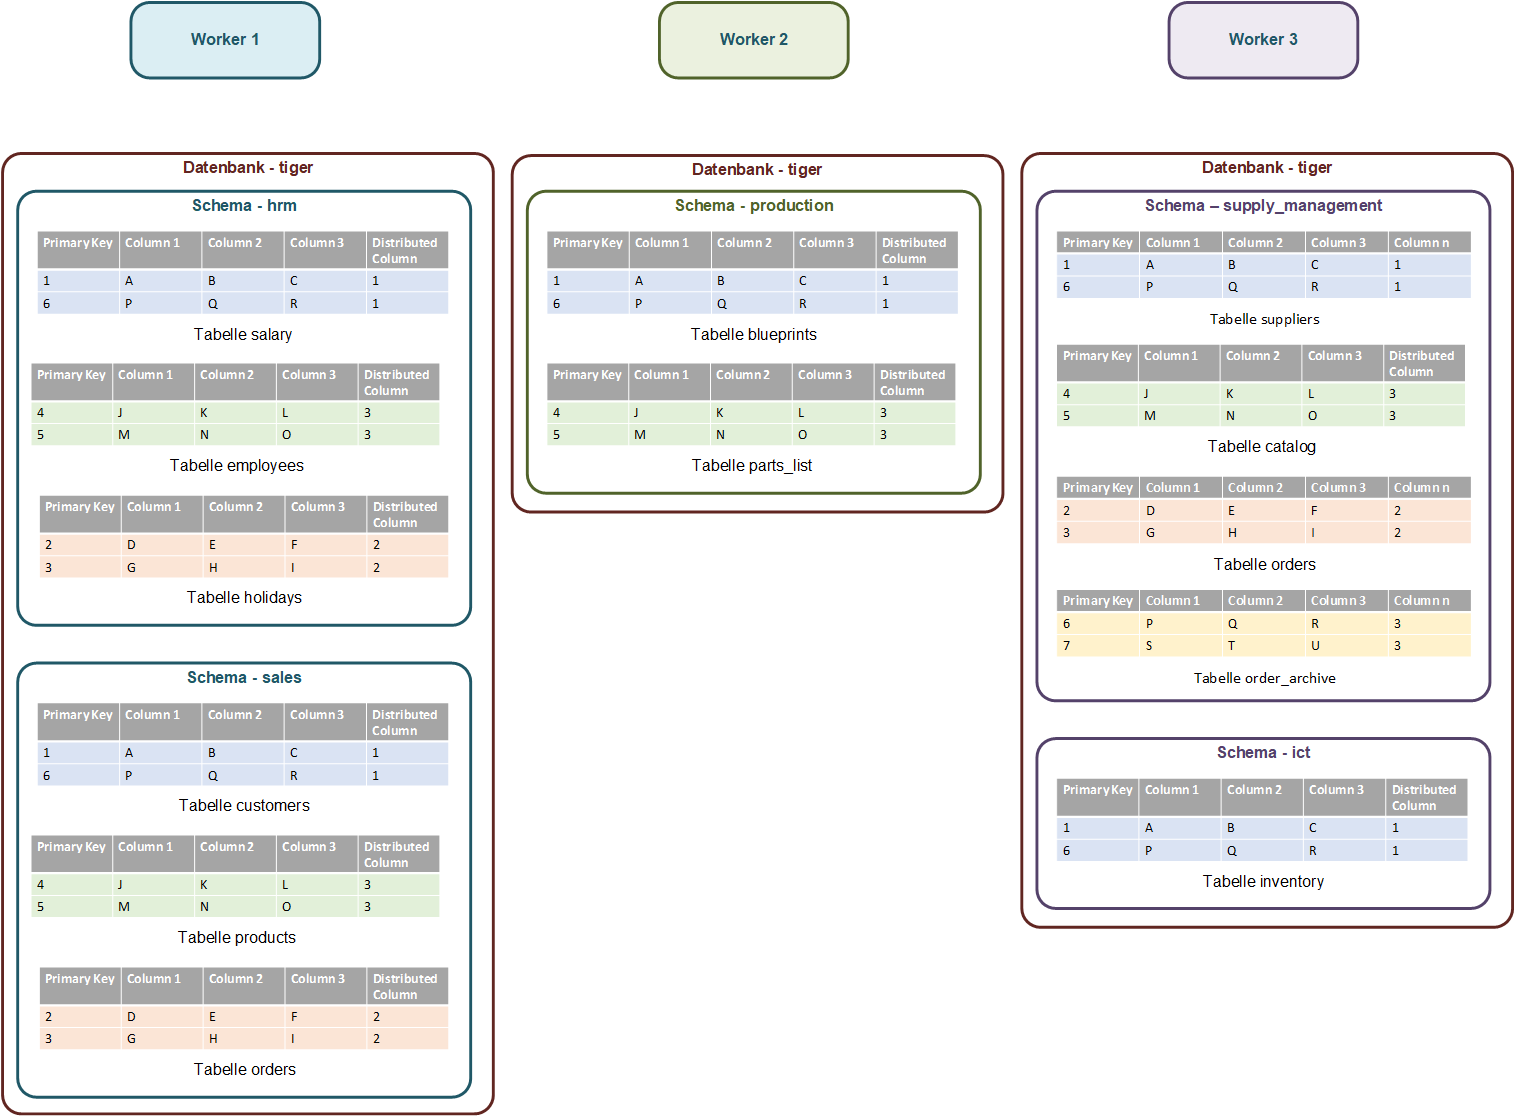
\includegraphics[width=0.8\linewidth]{source/implementation/evaluation/postgresql_ha_solutions/stackgres/citus_schema-based-sharding}
                \caption{Citus - Schema-Based-Sharding}
                \label{fig:citus_schema-based-sharding}
            \end{figure}
        \end{flushleft}
        \begin{flushleft}
            \textbf{Schlussfolgerung}
            Beide Sharding-Methoden haben eine grosse Schwäche.
            In Version 7.2 konnte noch ein Replikationsfaktor angegeben werden\cite{8W58EW47}, ab Version 11 wurde auch diese Variante gestrichen und man konnte noch eine 1:1 Repliacation auf einen Worker fahren\cite{JWYDYYWQ}.\\
            Spätestens mit Version 12 steht auch dies nicht mehr zur verfügung, man muss eine Replication auf e
%            Sie sind nicht vollständig ACID-Konform (\autoref{subsubsec:acid}) da Datenverlust entstehen kann, wenn ein Node wegfällt.
            Sie sind nicht vollständig ACID-Konform da Datenverlust entstehen kann, wenn ein Node wegfällt.
            Dies muss aber bei der evaluation mittels Tests noch bestätigt werden.
        \end{flushleft}
        \begin{flushleft}
            Die Shards müssen aber, stand heute, mit entsprechenden mit Replikation gesichert werden\cite{4GDXA49I}.\\
            Daraus ergibt sich aber ein nicht zu vernachlässigbarer Mehraufwand, wenn man self-healing Nodes implementieren möchte.\\
            Jeder Node ist für sich genommen, eine eigene Zone, um sicherzustellen, dass es zu keinem Datenverlust kommt,\\
            müsste jeder Shared-Node in eine der jeweiligen Zonen repliziert werden.\\
            Das heisst, es müssten \(Shard-Nodes^2 \) Replika-Nodes erstellt werden, hier ein Schematisches-Beispiel mit drei Shard-Nodes:
            \begin{figure}[H]
                \centering
                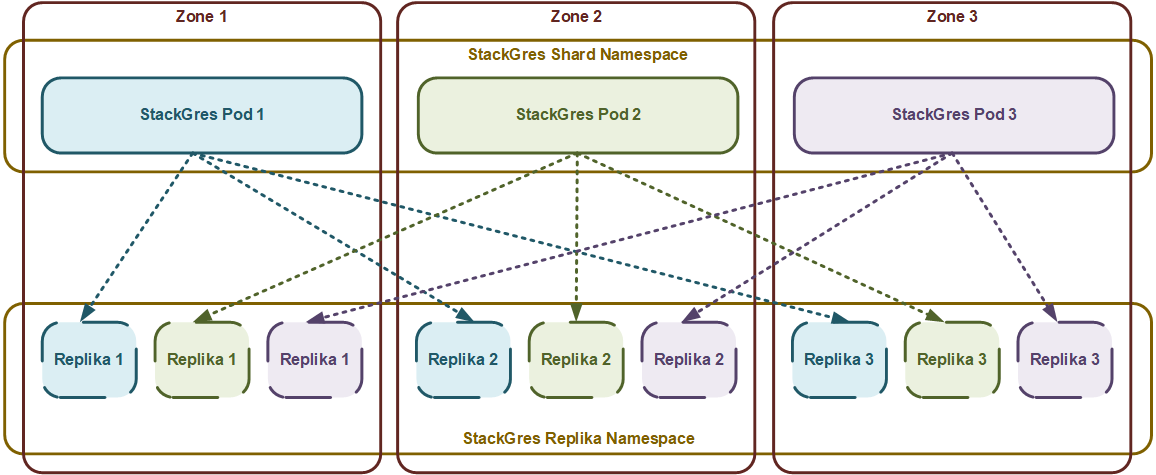
\includegraphics[width=0.8\linewidth]{source/implementation/evaluation/postgresql_ha_solutions/stackgres/stackgres_shard_replication}
                \caption{StackGres-Citus - Shard-Replikation}
                \label{fig:stackgres_shard_replication}
            \end{figure}
            Die Automation und nur schon die Konfiguration für das Mitskalieren, dürfte einiges an Zeit in Anspruch nehmen.\\
            Eine nicht unwesentliche folge, wäre ein starker Rückgang des Throughput's und Performance-Einbussen.
        \end{flushleft}
        \begin{flushleft}
            Alternativ kann natürlich ein Klassischer Replika-Server verwendet werden, wo die ganze Datenbank gesichert wird.\\
            Bis alle Daten wieder in den StackGres-Citus-Cluster zurückgeholt wurden, das Re-Balancing abgeschlossen ist usw.,\\
            muss der ganze Cluster für die User unerreichbar sein, da dieser in dieser Zeit nicht mehr konsistent ist.
        \end{flushleft}
        \begin{flushleft}
            Dieser zweite Ansatz bietet zwar Vorteile beim Throughput, doch im fehlerfall ist ein HA-Betrieb nur noch begrenzt garantiebar.
        \end{flushleft}
    \end{flushleft}
\end{flushleft}
\begin{flushleft}
    \paragraph{Maintenance}
    \hyperref[subsec:maintenance_stackgres_citus]{Anhang - Maintenance}
\end{flushleft}